\chapter{Graph RAG}

Sebbene la RAG tradizionale sia eccellente nel recuperare documenti basandosi sulla similarità semantica tramite database vettoriali,
si scontra frequentemente con una fisiologica perdita di contesto. I modelli vettoriali, infatti, faticano nel multi-hop reasoning,
ovvero nella capacità di estrarre e dedurre relazioni tra concetti distanti all'interno di un vasto corpus documentale.
Questo porta spesso a risposte incomplete o fuorvianti, specialmente quando le connessioni tra le informazioni non sono esplicitate nel testo.

Per arginare questo problema, è stato formalizzato il concetto di GraphRAG, un paradigma che sostituisce o affianca i vettori ai Knowledge Graph (KGs),
permettendo così di mappare in modo esplicito le entità e le loro interrelazioni. Tuttavia, l'implementazione originale di GraphRAG si rivela fortemente
"LLM-centrica", introducendo nuove criticità architetturali. Demandare a un Large Language Model l'intera costruzione del grafo e la sua successiva interrogazione —
ad esempio costringendolo a tradurre a runtime il linguaggio naturale in query Cypher — espone il sistema al rischio di allucinazioni sintattiche,
inconsistenze ontologiche e a un'impennata insostenibile dei costi di inferenza su larga scala.

La soluzione ingegneristica proposta supera questi colli di bottiglia integrando un database vettoriale (Qdrant) con un database a grafo (Neo4j),
facendoli comunicare attraverso la condivisione di identificatori univoci.

\newpage

\noindent
Il ciclo di vita del dato all'interno di questo sistema si divide in due macro-fasi. Durante l'inserimento dei dati (Ingestion),
i testi grezzi vengono elaborati — tramite LLM o tecniche di Named Entity Recognition — per estrarne un'ontologia strutturata di entità e relazioni,
che viene archiviata nel database a grafo Neo4j. Parallelamente, gli stessi documenti vengono convertiti in embedding vettoriali e memorizzati in Qdrant.
In questo modo, il sistema si assicura che la medesima informazione sia esplorabile sia da un punto di vista puramente semantico sia strutturale.

La vera sinergia tra le due tecnologie si esprime nella fase di recupero e generazione (Retrieval \& Generation). Quando l'utente pone una domanda,
il sistema non cerca di tradurla direttamente in linguaggio per i grafi, ma esegue prima una veloce ricerca vettoriale su Qdrant.
Questo passaggio permette di isolare in modo efficiente i frammenti di testo semanticamente più pertinenti. Una volta ottenuti gli ID di questi documenti,
il sistema li utilizza come punto di ingresso per interrogare Neo4j: il database a grafo recupera le reti relazionali associate a quegli ID,
espandendo il contesto con i nodi adiacenti e le loro connessioni esplicite.

\begin{figure}[htbp]
  \centering
  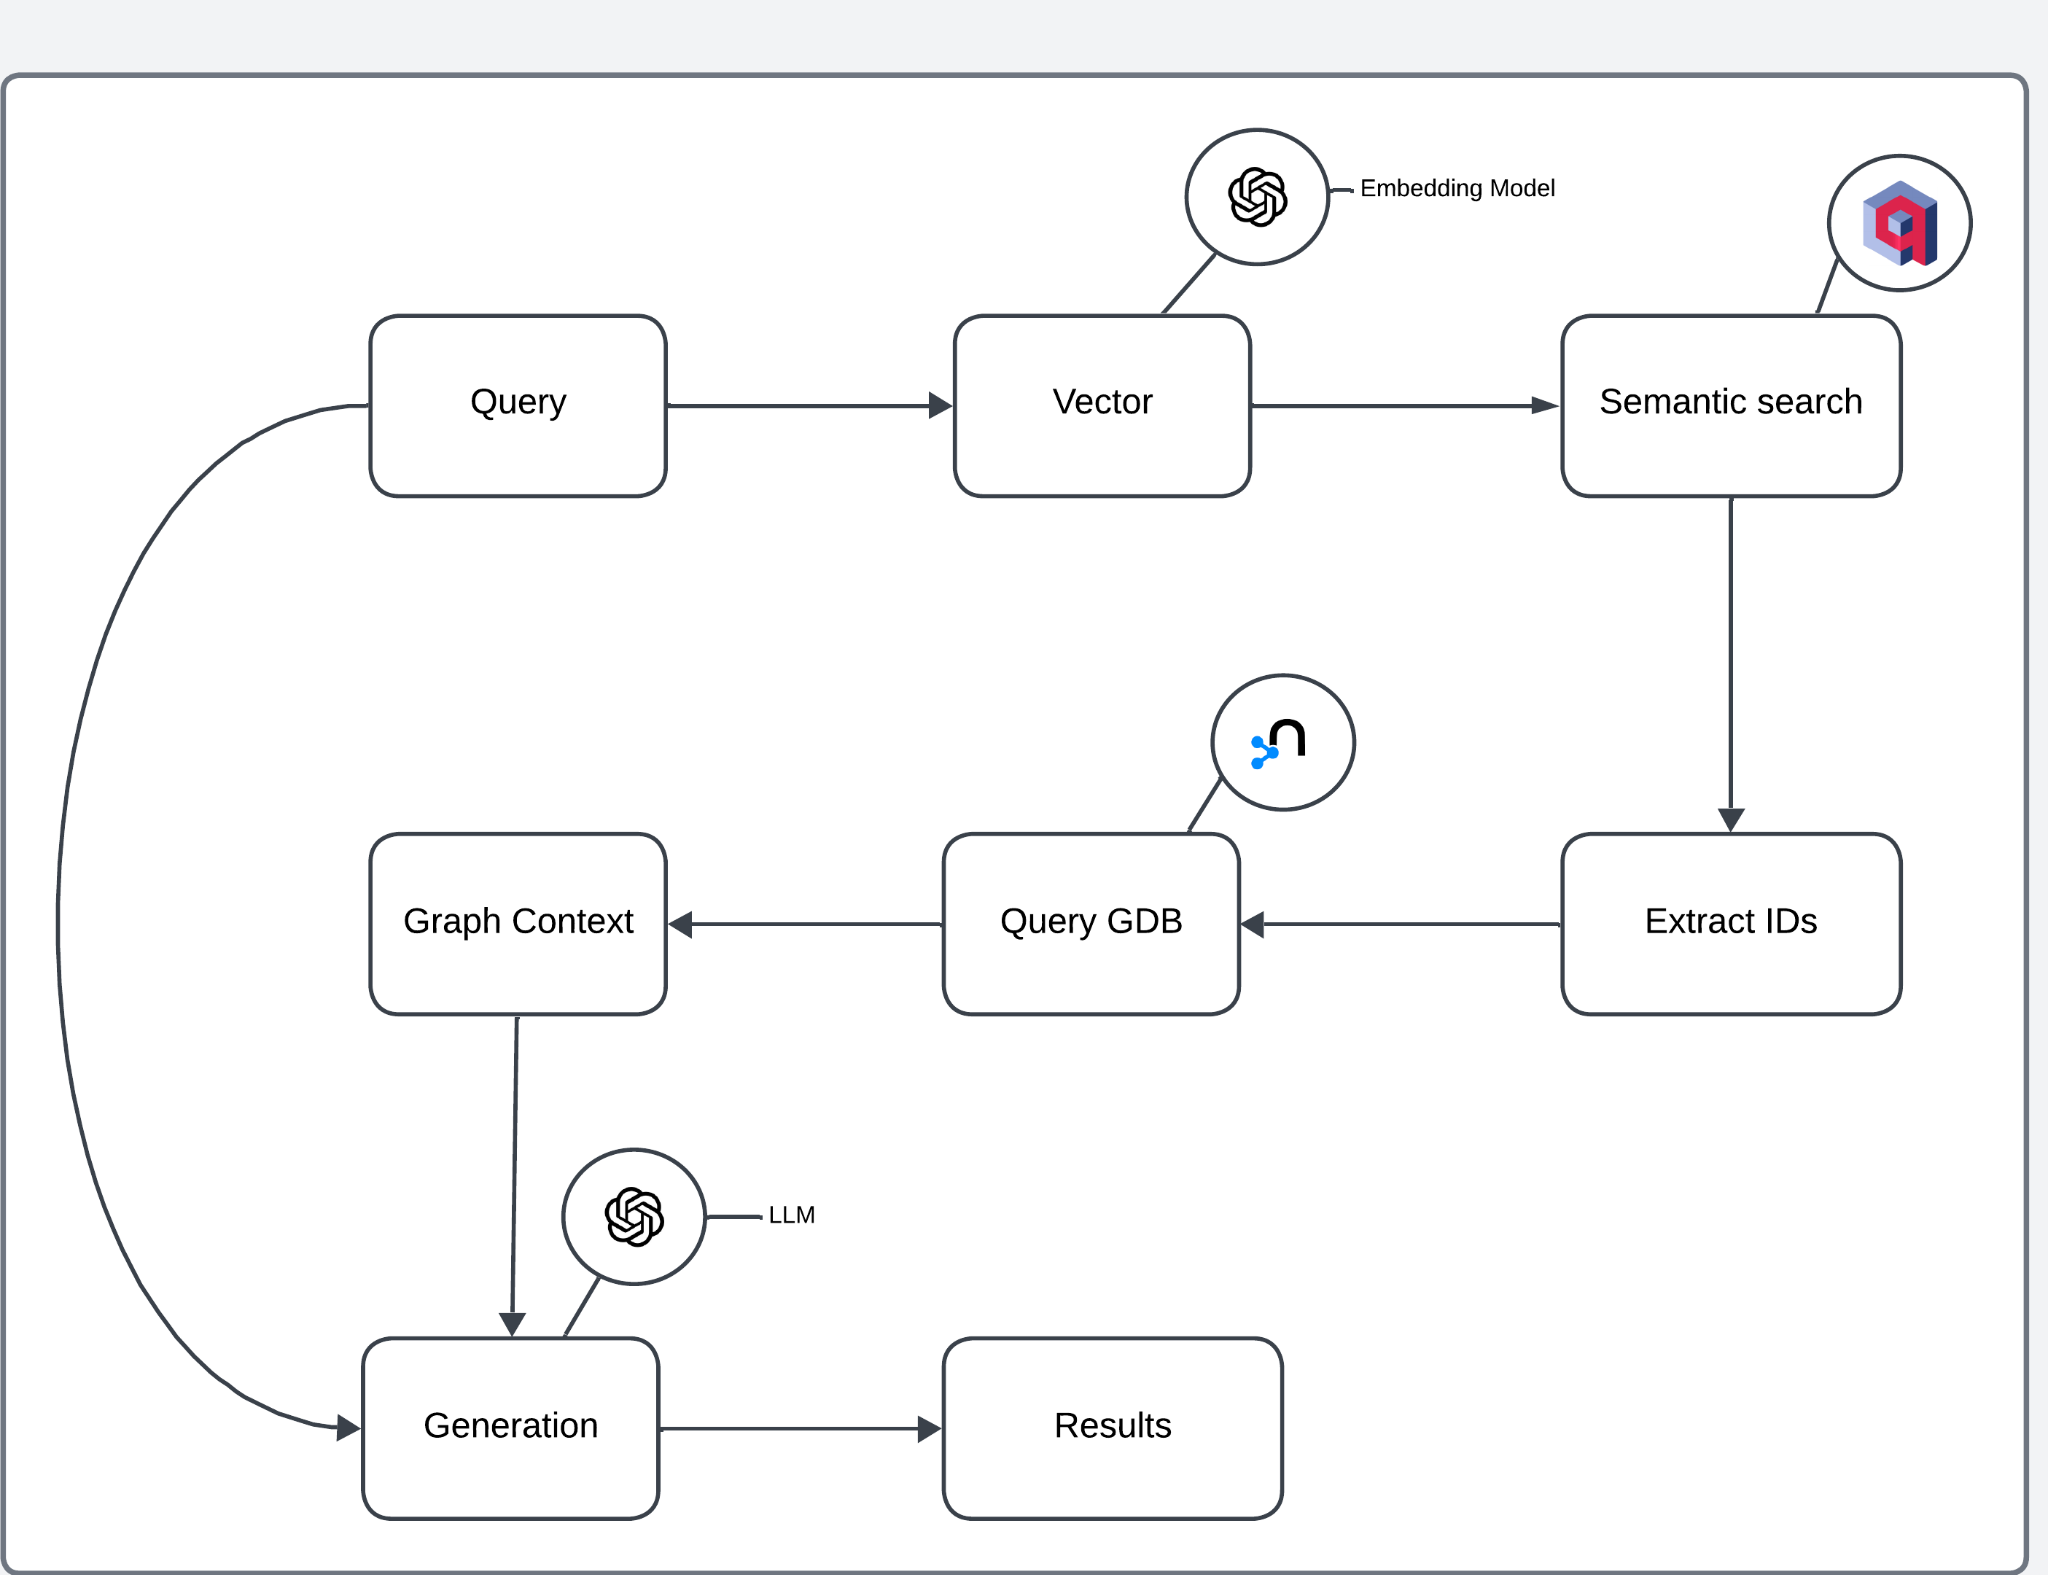
\includegraphics[width=0.7\textwidth]{images/graph_rag.png}
  \caption{grafo RAG}
  \label{fig:graph RAG}
\end{figure}

\noindent
Il risultato finale è un contesto ibrido, denso e deterministico, che viene fornito all'LLM per la generazione della risposta.
In un'ottica di architettura del software, il valore centrale di questo approccio per una tesi di informatica risiede nel principio di disaccoppiamento
delle responsabilità. Qdrant gestisce agilmente il matching semantico, Neo4j garantisce il rigore del contesto relazionale e l'LLM viene sollevato dal ruolo
inappropriato di "motore di interrogazione", tornando a fungere esclusivamente da generatore linguistico. Questo paradigma ibrido abbatte i costi computazionali,
azzera gli errori di querying dinamico e garantisce un'affidabilità delle risposte notevolmente superiore rispetto agli approcci monolitici. \cite{graph_rag}

\newpage

\section{Database vettoriali}
I database vettoriali rappresentano un'evoluzione fondamentale per l'Intelligenza Artificiale moderna. Essi sono progettati per memorizzare,
indicizzare e interrogare dati rappresentati sotto forma di embedding, ovvero vettori numerici ad alta dimensionalità generati da modelli di machine learning.
A differenza dei tradizionali motori di ricerca basati su keyword matching, i vector database operano attraverso la ricerca per similarità spaziale
(es. similarità del coseno, distanza euclidea o prodotto interno). Due concetti semanticamente affini si troveranno vicini all'interno dello spazio vettoriale,
indipendentemente dai termini specifici utilizzati per descriverli.

Nel contesto della nostra architettura, Qdrant ricopre l'incarico cruciale di motore di Semantic Search. Il suo compito è elaborare dati originariamente
non strutturati (es. le descrizioni in linguaggio naturale dei prodotti) e mapparli vettorialmente. Quando il sistema riceve una query,
Qdrant agisce come primo livello di filtraggio: isola in tempi dell'ordine dei millisecondi i frammenti informativi o i prodotti che presentano
la maggiore vicinanza semantica alla richiesta dell'utente. Qdrant eccelle nel gestire l'ambiguità del linguaggio naturale, individuando il "punto di ingresso"
ideale per la ricerca, ma, per sua natura, non possiede la consapevolezza strutturale di come tali informazioni siano collegate tra loro in un dominio complesso.

\section{Database a Grafo}
Per sopperire alla mancanza di contesto relazionale dei vettori, entrano in gioco i database a grafo. Questa tecnologia basa la propria architettura
sulla teoria dei grafi, abbandonando il rigido schema a tabelle dei database relazionali per modellare l'informazione attraverso nodi (le entità fisiche o logiche),
archi (le relazioni esplicite che collegano le entità) e proprietà. Il paradigma a grafo eccelle laddovebil valore dell'informazione risiede primariamente
nelle interconnessioni tra i dati.

Nel nostro sistema, Neo4j costituisce l'ossatura logica e relazionale dell'applicazione. A valle del processo di estrazione (operato da modelli come SAM3),
Neo4j immagazzina l'ontologia del dominio: istanzia i prodotti come nodi e crea un reticolo denso di archi che ne definiscono categorie, compatibilità,
specifiche tecniche e logiche di accoppiamento. Il principale vantaggio prestazionale di Neo4j è l'elaborazione Index-Free Adjacency:
le operazioni di attraversamento del grafo avvengono in tempo reale, poiché ogni nodo mantiene puntatori fisici diretti ai nodi adiacenti.
Ciò rende Neo4j lo strumento perfetto per il multi-hop reasoning, ovvero la capacità di estrarre percorsi logici complessi con una latenza minima,
indipendente dalle dimensioni totali del database.

\section{Integrazione di SAM3}

Come discusso in precedenza in merito all'architettura ibrida, il modello SAM3 svolge un ruolo cruciale all'interno del sistema,
fungendo da motore d'inferenza principale per la fase di popolamento (o ingestion) del database a grafo, che in questa implementazione è Neo4j.
Nello specifico, le avanzate capacità di analisi di SAM3 vengono impiegate per processare i dati in ingresso ed estrarre, con un elevato grado di precisione,
tutte le entità e le caratteristiche salienti pertinenti al dominio applicativo in esame.

Questo processo di estrazione mirata permette di tradurre informazioni eterogenee in un'ontologia ben definita e pronta per l'archiviazione strutturata.
Una volta isolati, gli elementi estratti vengono mappati e memorizzati all'interno dell'istanza di Neo4j: i prodotti di interesse vengono istanziati sotto forma
di nodi, mentre le loro peculiarità, i metadati e le reciproche interdipendenze vanno a costituire gli archi (relazioni).
Questa mappatura sistematica e deterministica porta alla generazione di un catalogo prodotti completo e semanticamente interconnesso,
sfruttando a pieno i vantaggi di flessibilità e modellazione offerti da Neo4j rispetto ai tradizionali database relazionali.

La strutturazione dell'informazione all'interno di un property graph come Neo4j apre a scenari di elaborazione e interrogazione particolarmente avanzati.
In fase di ricerca (retrieval), il sistema è in grado di avvalersi della topologia della rete, permettendo di navigare le relazioni esplicite
— anche attraversando nodi multipli — per rispondere a query complesse con latenze estremamente ridotte.
Inoltre, l'adozione di Neo4j si rivela fondamentale per l'implementazione di logiche di "accoppiamento significativo". Analizzando i percorsi, le adiacenze
e i gradi di separazione tra i vari nodi, il sistema può dedurre connessioni semantiche non banali tra molteplici prodotti. Ciò abilita lo sviluppo di funzionalità
di alto livello, come i sistemi di raccomandazione context-aware, capaci di suggerire combinazioni di articoli basate su affinità strutturali e logiche di business
codificate direttamente all'interno della rete relazionale del grafo.